\documentclass[../main.tex]{subfiles}
\graphicspath{ {\subfix{../../img/}} }

\begin{document}
\section{Theory}

    MOSFETs [Metal-Oxide Semiconductor Field-Effect Transistors] are a type of transistors.
    MOSFETs consist of two groups, n-channel and p-channel, both of which seperate into two 
    as depletion and enhancement mode MOSFETs. This experiment will be focusing on 
    n-channel enhancement mode MOSFETs, and throughout this report, we will be mentioning 
    them as MOSFETs rather than clarifying the entire name.

    Phyical structure of the MOSFET as shown in Figure \ref{fig:structure} consists of a large 
    \textbf{body}, made out of positively doped semiconductor material, upon which two heavily 
    negatively doped regions are placed, called \textbf{source} and \textbf{drain}. Between these 
    two heavily doped regions, seperated from the body with an insulating material, a conducting 
    plate is placed, called the \textbf{gate}. 

    \begin{figure}[H]\centering
        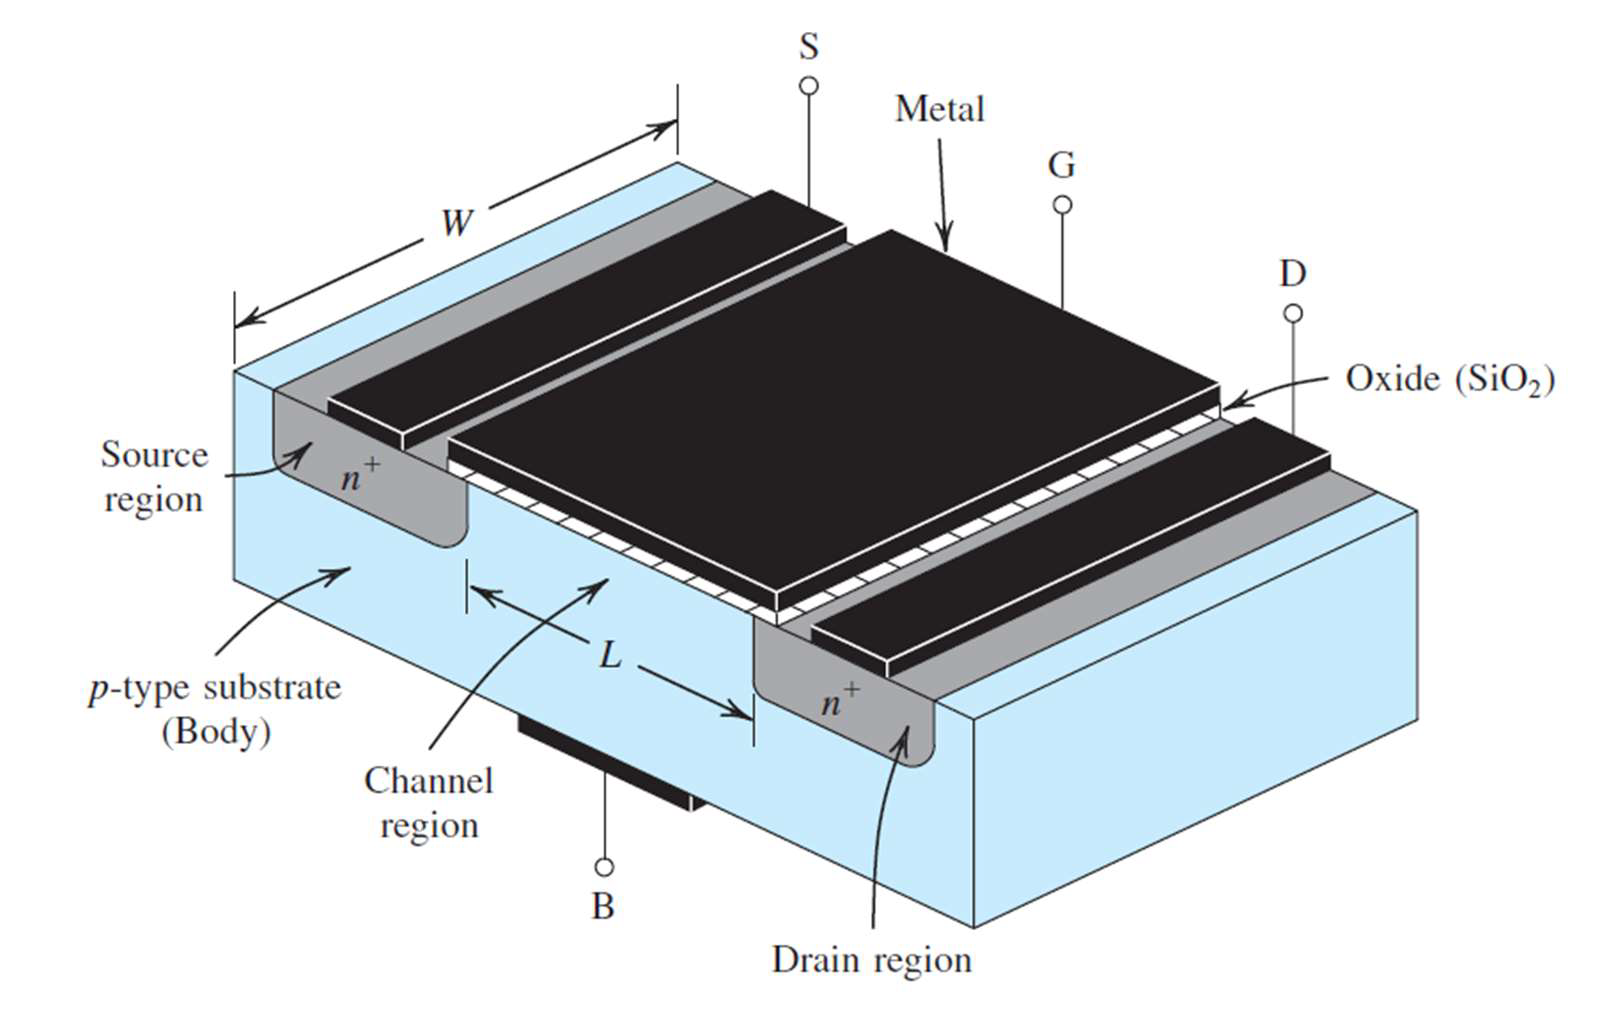
\includegraphics[width=0.7\textwidth]{structure.png}
        \caption{Physical structure of an n-channel enhancement mode MOSFET, [Sedra-Smith]}\label{fig:structure}
    \end{figure}

    As can be seen, both drain and source forms a PN junction 
    with the body, in opposite direction with respect to each other. Hence, if a voltage of either polarity were 
    to be applied to drain and source, one of these PN junctions will be reverse biased, blocking any current flow
    between drain and the source.\footnotemark This region is called the \textbf{cut-off} region, with very high effective 
    resistance between drain and source.
    \footnotetext{Ignoring junction breakdowns.}

    Suppose for simplicity, the body and the source are tied together,\footnote{As it usually is for discrete MOSFETs, though rarely is for IC MOSFETs.} 
    and every voltage is referanced from this potential.
    If a sufficiently high positive voltage is to be applied to the gate, the electric field created by this voltage 
    between the gate plate and the body pulls electrons from the body and towards itself. This results in a high electron
    concentration between the drain and the source, essentially creating a channel filled with electrons between two 
    negatively doped regions, thus creating a path for current to flow between the drain and source. This \textit{sufficiently high}
    voltage is called \textbf{threshold voltage}, albeit, a bit ambigiously. For instance, the gate threshold voltage 
    \textbf{$V_{GS_{(th)}}$} denotes a voltage applied to the gate that allows an arbitrary but sufficient current flow 
    from drain to source, at a specific drain voltage. \textbf{Zero bias threshold voltage $V_{0_{th}}$} denotes 
    the voltage required to fully form the channel.
    
    \begin{figure}[H]\centering
        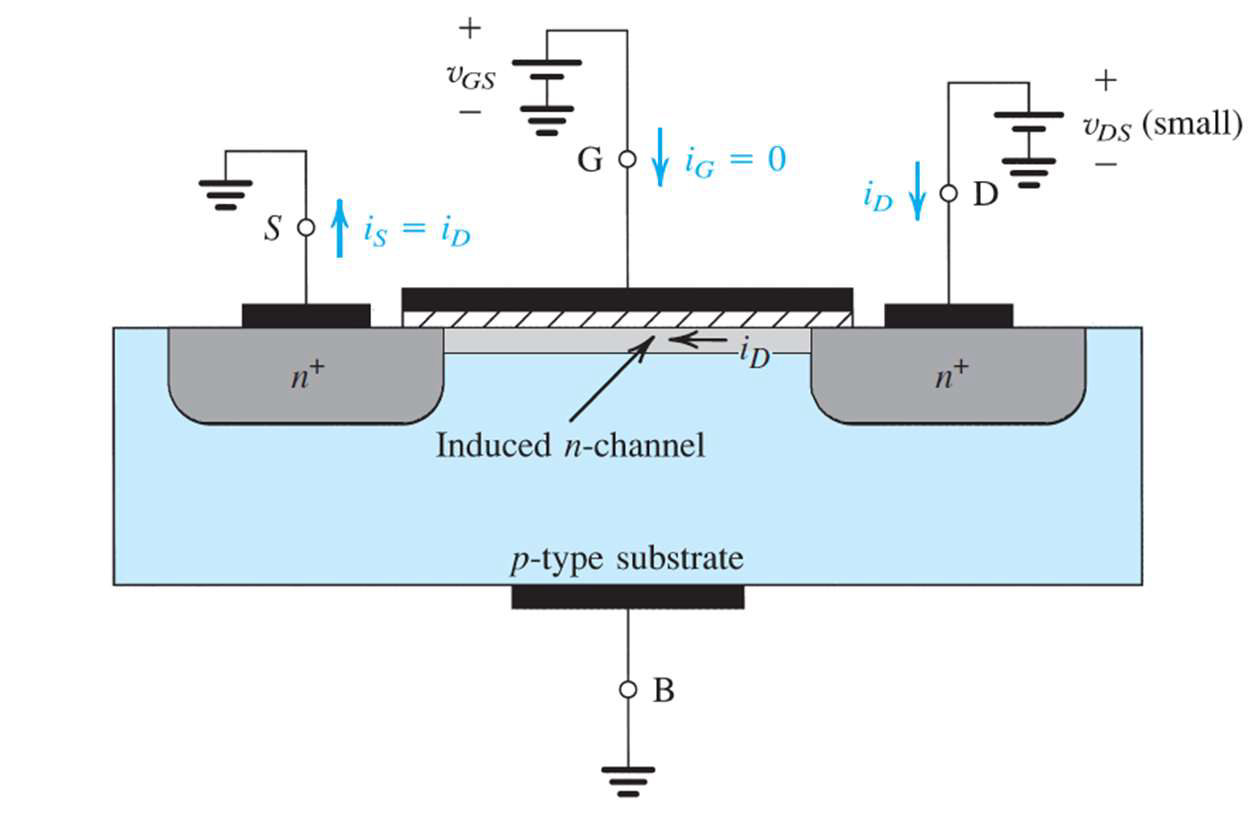
\includegraphics[width=0.7\textwidth]{channel.png}
        \caption{}\label{fig:channel}
    \end{figure}

    Either way, as the channel created, applying a small positive voltage at the drain results in an appreciable current flow. 
    This \textbf{drain current}, or drain to source current, for relatively small drain voltage, appears to be linearly proportional to the 
    drain voltage, hence the MOSFET behaves like a voltage controlled resistor, where its resistance is inversly proportional 
    to the gate voltage, or more correctly, the difference between the gate voltage and the threshold voltage $V_{GS}-V_{th}$,
    which is conveniently named \textbf{overdrive voltage $V_{ov}$}. The relation is given below.

    \begin{equation}
        I_D = \left[\left(\mu_n C_{ox}\frac{W}{L}\right)\left(V_{GS}-V_{th}-\frac{1}{2}V_{DS}\right)\right]V_{DS}
    \end{equation}

    The factor consisting of many terms is a constant that is determined by the physical structure 
    of the MOSFET, let us define it as:

    \begin{equation}
        \kappa \triangleq \left(\mu_n C_{ox}\frac{W}{L}\right)
    \end{equation}

    \noindent Then the expression looks simpler as:

    \begin{equation}
        I_D = \kappa\left(V_{GS}-V_{th}-\frac{1}{2}V_{DS}\right)V_{DS}
    \end{equation}

    Which is a downward looking parabola. If we were to 
    treat the $V_{GS}$ as a constant, it can be seen that for sufficiently small $V_{DS}$, it looks like a line with 
    its slope controlled by $V_{GS}$, and hence the voltage controlled resistor. This region, rather deceptively called
    the \textbf{linear region}, or the triode region.

    \begin{figure}[H] \centering
            \begin{tikzpicture}
                \begin{axis}
                [
                    standard,
                    scale = 1,
                    height = 0.4\textwidth,
                    width = 0.7\textwidth,
                    %axis lines = middle,
                    xlabel = {$V_D$},
                    ylabel = {$I_D$},
                    xticklabels = {,,},
                    yticklabels = {,,},
                    xmin = -0.5, xmax = 5,
                    ymin = -0, ymax = 260,
                    %xtick={-1,0,1,2,3,4,5},
                    %ytick={-1,0,1,2,3,4,5},
                    minor tick num = 1
                ]
                    \addplot
                    [
                        domain = 0:4,
                        samples = 100,
                        thick,
                        blue,
                    ]{ 20*( 7 - 1 - 0.5*x)*x }{};
                    \addplot
                    [
                        domain = 0:5,
                        samples = 100,
                        thick,
                        blue,
                    ]{ 20*( 6 - 1 - 0.5*x)*x }{};
                    \addplot
                    [
                        domain = 0:4,
                        samples = 100,
                        thick,
                        blue,
                    ]{ 20*( 5 - 1 - 0.5*x)*x }{};
                    \addplot
                    [
                        domain = 0:3,
                        samples = 100,
                        thick,
                        blue,
                    ]{ 20*( 4 - 1 - 0.5*x)*x }{};
                \end{axis}
            \end{tikzpicture}
        \caption{Linear Region Drain Current Curves, increasing $V_{GS}$ at ccw.}\label{cclin}
    \end{figure}

    It can be seen from the example plot that $I_D$ loses its linear looking property as $V_{DS}$ increases. Since 
    the positive voltage applied to the drain, decreases the potential difference between the gate and the body near the 
    drain, the channel narrows towards the drain, hence increasing the effective resistance between drain and source.
    This proportional increase in the effective resistance cannot be neglected for relatively large drain voltages.

    As the curve flattens, as the parabola reaches its maximum, i.e., $V_{DS} = (V_{GS}-V_{th})$, the MOSFET enters 
    anoter mode of operation, called the \textbf{saturation}. Here, the drain voltage increased such that the channel
    at the drain end has 0 thickness, called \textit{channel pinch-off}. It is assumed that beyond this point,
    $V_{DS}$ has no effect on the drain current, (channel cannot have a negative thickness, right?). Thus the 
    drain current remains constant for $V_{DS}$ above this value, or $V_{DS_{(sat)}}$. 

    \noindent The expression for drain current in this region is as follows.
    \begin{equation}
        I_D = \frac{1}{2}\kappa\left(V_{GS}-V_{th}\right)^2
    \end{equation}

    Here, the drain current is no longer a function of $V_{DS}$, hence will appear as constant against $V_{DS}$, and 
    is a quadratic function of $V_{GS}$. In other words, the MOSFET behaves like an ideal current source, albeit, a 
    non-linear one.
    \begin{figure}[H]\centering
        \begin{circuitikz}
            
            \draw
            (0,1.5) node[nigfete](mos){}
            (mos.G) -| ++(-1,0) node[ocirc, left](G){G}
            (mos.D) |- ++(0,1) node[ocirc, above](D){D}
            (mos.S) |- ++(0,-1) node[ocirc, below](S){S}

            (G) to[open, v=$V_{GS}$] (S)
            (D) ++(1,0) to[open, v^=$V_{DS}$] (1,0) ++(S)
            ;
            \draw(3.25,1.5) node[left]{$\equiv$};

            \draw
            (5,0)   
                    to[open, v<=$V_{GS}$, o-o] (5,3) -- (6,3)
                    to[open, o-o] (11,0) -- (5,0)
            (9,0)
                    to[cI, l=$\frac{1}{2}\kappa(V_{GS}-V_{th})^2$, invert] (9,3)
                    to[short, -o] (11,3)
                    to[open, v=$V_{DS}$] (11,0)
            (8,0)node[below]{S}
            ;

        \end{circuitikz}
        \caption{Equivalent ideal circuit for an NMOS operating at saturation region. $V_{DS}<(V_{GS}-V_{th})$}\label{fig:equiv1}
    \end{figure}

    % Ideal $I_D-V_{DS}$ and $I_D-V_{GS}$ Characteristics
    \begin{figure}[H] \centering
        \subfloat[$I_D-V_{DS}$ graph, linear-saturation regions.]
        {%
            \begin{tikzpicture}
                \begin{axis}
                [
                    standard,
                    scale = 1,
                    height = 0.4\textwidth,
                    width = 0.6\textwidth,
                    %axis lines = middle,
                    xlabel = {$V_D$},
                    ylabel = {$I_D$},
                    xticklabels = {,,},
                    yticklabels = {,,},
                    xmin = -0.5, xmax = 10,
                    ymin = -0, ymax = 280,
                    %xtick={-1,0,1,2,3,4,5},
                    %ytick={-1,0,1,2,3,4,5},
                    minor tick num = 1
                ]
                    \addplot
                    [
                        domain = 0:10,
                        samples = 100,
                        thick,
                        blue,
                    ]
                    {
                        (20*( 6 - 1 - 0.5*x)*x)*(x<5) + (0.5*20*(6-1)^2*(x>=5))     
                    }{};
                    \addplot
                    [
                        domain = 0:10,
                        samples = 100,
                        thick,
                        blue,
                    ]
                    {
                        (20*( 5 - 1 - 0.5*x)*x)*(x<4) + (0.5*20*(5-1)^2*(x>=4))     
                    }{};
                    \addplot
                    [
                        domain = 0:10,
                        samples = 100,
                        thick,
                        blue,
                    ]
                    {
                        (20*( 4 - 1 - 0.5*x)*x)*(x<3) + (0.5*20*(4-1)^2*(x>=3))     
                    }{};
                    \addplot
                    [
                        domain = 0:10,
                        samples = 100,
                        thick,
                        black,
                        dashed,
                    ]
                    {
                        (0.5*20*(x)^2     
                    }{};

                \end{axis}
            \end{tikzpicture}
        }
        \qquad
        \subfloat[$I_D-V_{GS}$ graph, \textbf{on saturation region}.]
        {%
            \begin{tikzpicture}
                \begin{axis}
                [
                    standard,
                    scale = 1,
                    height = 0.4\textwidth,
                    width = 0.4\textwidth,
                    %axis lines = middle,
                    xlabel = {$V_G$},
                    ylabel = {$I_D$},
                    xticklabels = {,,},
                    yticklabels = {,,},
                    xmin = -0.5, xmax = 5,
                    ymin = -0, ymax = 180,
                    %xtick={-1,0,1,2,3,4,5},
                    %ytick={-1,0,1,2,3,4,5},
                    minor tick num = 1
                ]
                    \addplot
                    [
                        domain = 0:10,
                        samples = 100,
                        thick,
                        blue,
                    ]
                    {
                        (x>=1)*(0.5*20*(x-1)^2 + 0    
                    }{};
                \end{axis}
            \end{tikzpicture}
        }

        \caption{Ideal $I_D-V_{DS}$ and $I_D-V_{GS}$ Characteristics}\label{inf_ro.gph}
    \end{figure}

    Combining these three cases, three regions of operation, a full expression for the drain current is as follows.

    \begin{equation}
        I_D = 
        \begin{cases}
            0, &V_{GS}<V_{th}\\
            \kappa\left(V_{GS}-V_{th}-\frac{1}{2}V_{DS}\right)V_{DS}, &V_D \leq (V_{GS}-V_{th})\\
            \frac{1}{2}\kappa(V_{GS}-V_{th})^2, &V_{DS} > (V_{GS}-V_{th})
        \end{cases}
        \quad \kappa \triangleq \left(\mu_n C_{ox}\frac{W}{L}\right)
    \end{equation}

    \pagebreak
    Of course, those perfectly constant drain currents looks a bit too good to be true. It was said that increasing 
    the $V_{DS}$ beyond $V_{DS_{(sat)}}$ would not have any effect. It, however, does. Increasing the $V_{DS}$ beyond 
    that causes the \textit{pinched-off} point of the channel to seperate and move away from the drain, while it still
    maintains the conduction, it reduces the output resistance of the MOSFET from infinite to a finite value. To encompansate 
    this effect, the equation can be modified as below, where $\lambda$ is a device parameter in $\SI{}{\per\volt}$.

    \begin{equation}
        I_D = 
        \begin{cases}
            0, &V_{GS}<V_{th}\\
            \kappa(1+\lambda V_{DS})\left(V_{GS}-V_{th}-\frac{1}{2}V_{DS}\right)V_{DS}, &V_D \leq (V_{GS}-V_{th})\\
            \frac{1}{2}\kappa(1+\lambda V_{DS})(V_{GS}-V_{th})^2, &V_{DS} > (V_{GS}-V_{th})
        \end{cases}
        %\quad \kappa \triangleq \left(\mu_n C_{ox}\frac{W}{L}\right)
    \end{equation}

    \begin{figure}[H]\centering
        \begin{circuitikz}
            \draw
            (0,0)   
                    to[open, v<=$V_{GS}$, o-o] (0,3) -- (1,3)
                    to[open, o-o] (9,0) -- (0,0)
            (4,0)
                    to[cI, l=$\frac{1}{2}\kappa(V_{GS}-V_{th})$, invert] (4,3)
                    to[short, -o] (9,3)
                    to[open, v=$V_{DS}$] (9,0)
            (6,3) to[R, l=$r_o {=} \frac{1}{\lambda I_{D(sat)}}$, *-*] (6,0)
            (3,0)node[below]{S}
            ;
            
        \end{circuitikz}
        \caption{Equivalent ideal circuit for an NMOS operating at saturation region. $V_{DS}<(V_{GS}-V_{th})$ \\With finite output resistance.}\label{fig:equiv2}
    \end{figure}

    % $I_D-V_{DS}$ and $I_D-V_{GS}$ Characteristics with finite output resistance
    \begin{figure}[H] \centering
        \subfloat[$I_D-V_{DS}$ graph, linear-saturation regions.]
        {%
            \begin{tikzpicture}
                \begin{axis}
                [
                    standard,
                    scale = 1,
                    height = 0.4\textwidth,
                    width = 0.6\textwidth,
                    %axis lines = middle,
                    xlabel = {$V_D$},
                    ylabel = {$I_D$},
                    xticklabels = {,,},
                    yticklabels = {,,},
                    xmin = -0.5, xmax = 10,
                    ymin = -0, ymax = 330,
                    %xtick={-1,0,1,2,3,4,5},
                    %ytick={-1,0,1,2,3,4,5},
                    minor tick num = 1
                ]
                %%%%% Original - Dashed Red %%%%%
                    \addplot[domain = 0:10, samples = 100, thick, red, dashed]
                    {
                        (20*( 6 - 1 - 0.5*x)*x)*(x<5) + (0.5*20*(6-1)^2*(x>=5))     
                    }{};

                    \addplot[domain = 0:10, samples = 100, thick, red, dashed]
                    {
                        (20*( 5 - 1 - 0.5*x)*x)*(x<4) + (0.5*20*(5-1)^2*(x>=4))     
                    }{};

                    \addplot[domain = 0:10, samples = 100, thick, red, dashed]
                    {
                        (20*( 4 - 1 - 0.5*x)*x)*(x<3) + (0.5*20*(4-1)^2*(x>=3))     
                    }{};
                %%%%%-----------------------%%%%%

                %%%% With output resistance %%%%%
                    \addplot[domain = 0:10, samples = 100, thick, blue]
                    {
                        (20*(1+0.025*x)*( 6 - 1 - 0.5*x)*x)*(x<5) + (0.5*20*(1+0.025*x)*(6-1)^2*(x>=5))     
                    }{};

                    \addplot[domain = 0:10, samples = 100, thick, blue]
                    {
                        (20*(1+0.025*x)*( 5 - 1 - 0.5*x)*x)*(x<4) + (0.5*20*(1+0.025*x)*(5-1)^2*(x>=4))     
                    }{};

                    \addplot[domain = 0:10, samples = 100, thick, blue, ]
                    {
                        (20*(1+0.025*x)*( 4 - 1 - 0.5*x)*x)*(x<3) + (0.5*20*(1+0.025*x)*(4-1)^2*(x>=3))     
                    }{};

                    %%%%%-------------------%%%%%
                    \addplot[domain = 0:10, samples = 100, thick, black, dashed]
                    {
                        (0.5*20*(1+0.025*x)*(x)^2     
                    }{};

                \end{axis}
            \end{tikzpicture}
        }
        \qquad
        \subfloat[$I_D-V_{GS}$ graph, \textbf{on saturation region}.]
        {%
            \begin{tikzpicture}
                \begin{axis}
                [
                    standard,
                    scale = 1,
                    height = 0.4\textwidth,
                    width = 0.4\textwidth,
                    %axis lines = middle,
                    xlabel = {$V_G$},
                    ylabel = {$I_D$},
                    xticklabels = {,,},
                    yticklabels = {,,},
                    xmin = -0.5, xmax = 5,
                    ymin = -0, ymax = 180,
                    %xtick={-1,0,1,2,3,4,5},
                    %ytick={-1,0,1,2,3,4,5},
                    minor tick num = 1
                ]
                    \addplot
                    [
                        domain = 0:10,
                        samples = 100,
                        thick,
                        red,
                        dashed
                    ]
                    {
                        (x>=1)*(0.5*20*(x-1)^2 + 0    
                    }{};
                    \addplot
                    [
                        domain = 0:10,
                        samples = 100,
                        thick,
                        blue,
                    ]
                    {
                        (x>=1)*(0.5*20*(1+0.025*x)*(x-1)^2 + 0    
                    }{};
                \end{axis}
            \end{tikzpicture}
        }

        \caption{$I_D-V_{DS}$ and $I_D-V_{GS}$ Characteristics with finite output resistance.
                 Ideal plots shown in dashed red.}\label{ro.gph}
    \end{figure}

    \pagebreak
    Lastly, recall that the gate was insulated from the body with an insulating layer, two conducting surfaces 
    seperated by an insulator, a capacitor! Of course, given the average size of these devices (structurally), 
    this capacitance will be quite small, but it's still going to be effecting the operation of the MOSFET at high 
    frequencies or fast switching operations. Since we have connected the body and source together, this capacitance 
    appears between the gate and the source. What follows, of course, is another, smaller capacitance between the gate 
    and the drain, but its effects are not as obvious as the gate-source capacitance. The equivalent circuit model 
    can be improved by adding a capacitor into the input port.

    \begin{figure}[H]\centering
        \begin{circuitikz}
            \draw
            (-1,0)   
                    to[open, v<=$V_{GS}$, o-o] (-1,3) -- (0,3)
                    to[C, l=$C_{GS}$] (0,0)
                    to[open, o-o] (9,0) -- (-1,0)
            (5,0)
                    to[cI, l=$\frac{1}{2}\kappa(V_{GS}-V_{th})$, invert] (5,3)
                    to[short, -o] (9,3)
                    to[open, v=$V_{DS}$] (9,0)
            (6,3) to[R, l=$r_o {=} \frac{1}{\lambda I_{D(sat)}}$, *-*] (6,0)
            (3,0)node[below]{S}
            ;
            
        \end{circuitikz}
        \caption{Equivalent circuit for an NMOS operating at saturation region $V_{DS}<(V_{GS}-V_{th})$. \\With finite output resistance and gate-source capacitance. }\label{fig:equiv3}
    \end{figure}






\end{document}